\documentclass[12pt,a4paper,twoside]{report}
\usepackage{graphicx} % Required for inserting images
\usepackage[utf8]{inputenc}
%\usepackage[english]{babel}
\usepackage[portuguese]{babel}
\usepackage[margin=2.5cm]{geometry}
%\usepackage[toc,page]{appendix}
\usepackage[nottoc,numbib]{tocbibind}
\usepackage{pdfpages}
\usepackage{parskip}
\usepackage{url}
\usepackage[acronym]{glossaries}
\makeglossaries

\usepackage{listings}
\renewcommand{\lstlistingname}{Listagem}
\renewcommand*{\lstlistlistingname}{Lista de Listagens}
\lstset{
 xleftmargin = 1cm,
 basicstyle=\footnotesize, 
 numbers=left, 
 captionpos=b,
 columns=fullflexible,
 breaklines=true,
 frame=single
}

\begin{document}
%substituir pela versão preenchida
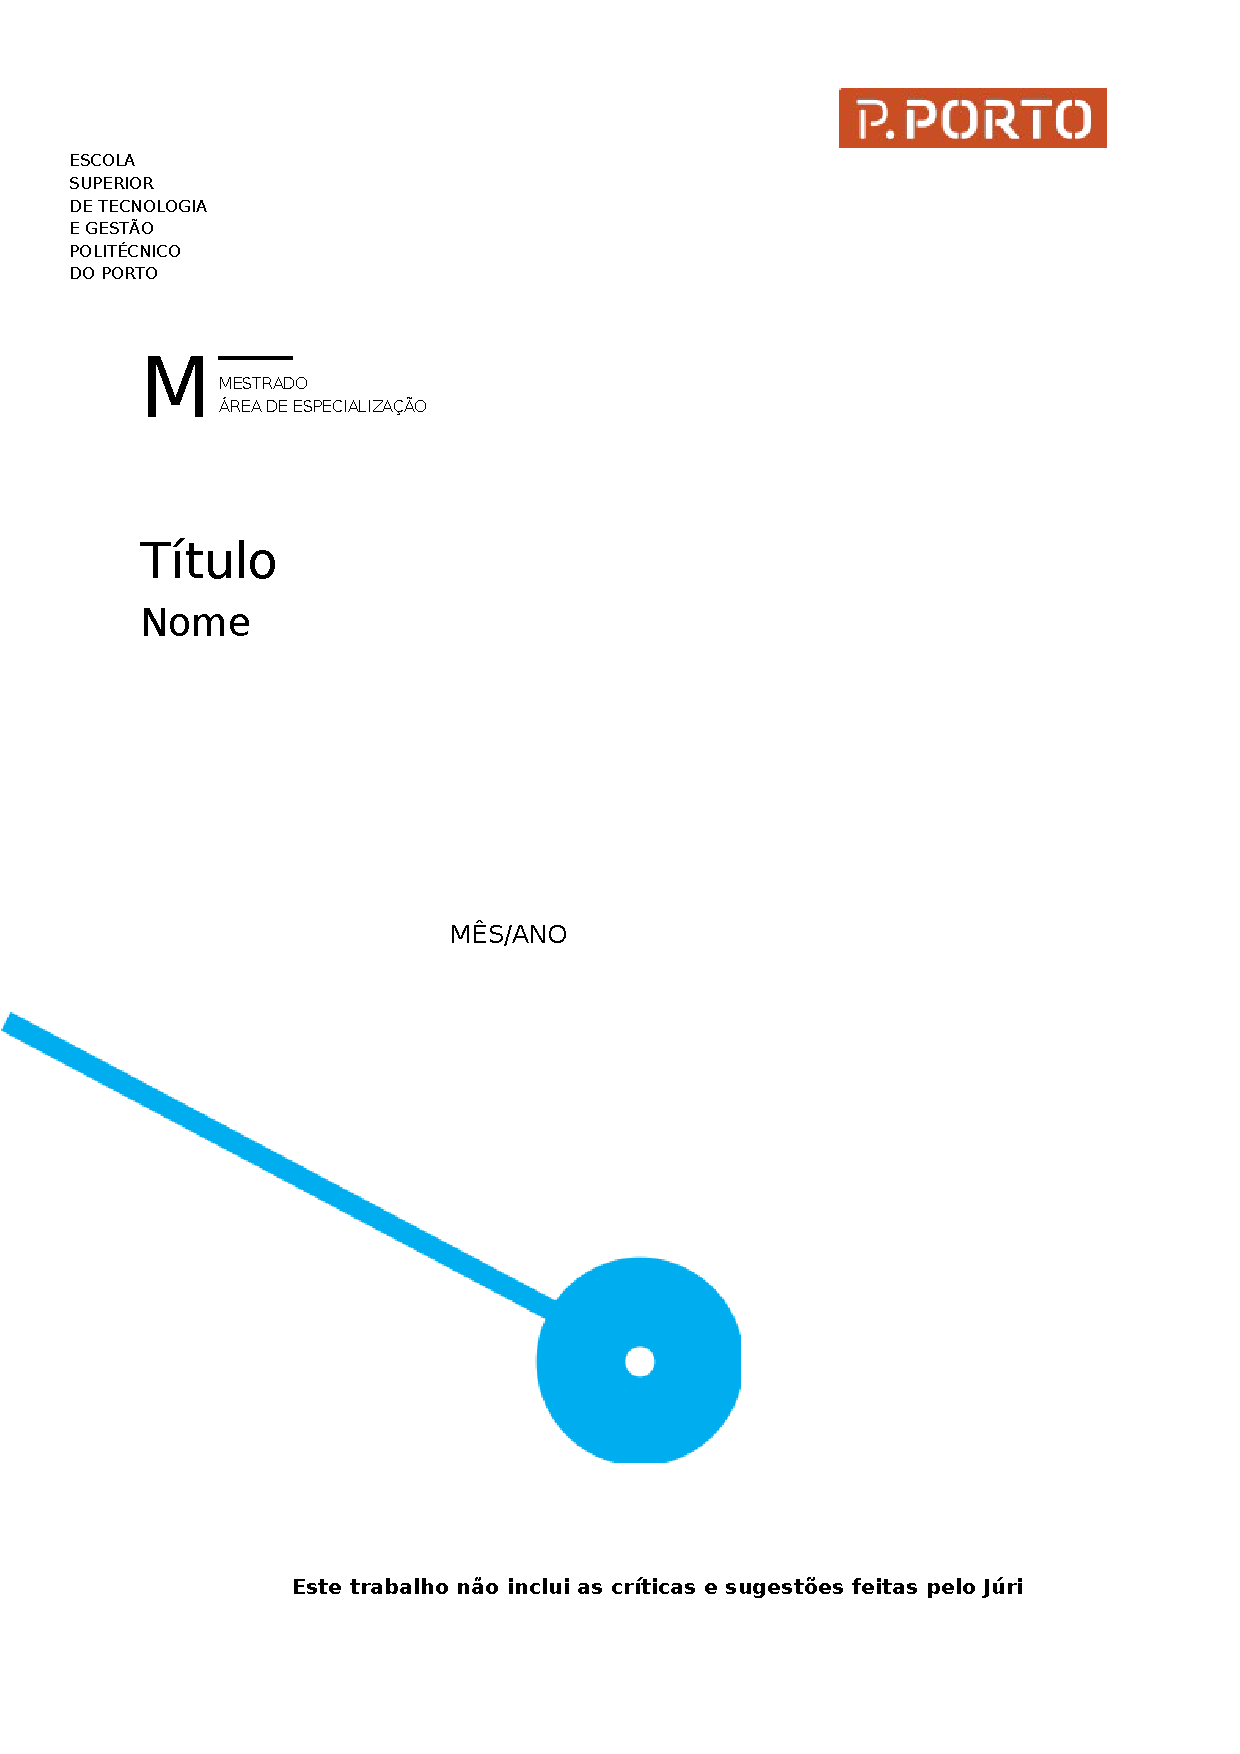
\includepdf[pages=1-2]{capas/capa.pdf}
\pagenumbering{roman}
%%%% colocar aqui acrónimos
\newacronym{estg}{ESTG}{Escola Superior de Tecnologia e Gestão}

\chapter*{Declaração de integridade}

Eu, \textbf{NOME DO ESTUDANTE}, estudante nº \textbf{8888888}, do Mestrado \textbf{NOME DO MESTRADO} da Escola Superior de Tecnologia e Gestão do Instituto Politécnico do Porto, declaro que não fiz plágio nem auto-plágio, pelo que o trabalho intitulado “\textbf{TITULO DA TESE}” é original e da minha autoria, não tendo sido usado previamente para qualquer outro fim. Mais declaro que todas as fontes usadas estão citadas, no texto e na bibliografia final, segundo as regras de referenciação adotadas na instituição.

\chapter*{Agradecimentos}
%Opcional, capítulo pode ser comentado

\chapter*{Abstract}
%Opcional, capítulo pode ser comentado

\textbf{Keywords:} Palavra1, Palavra 2, Palavra 3

\chapter*{Resumo}

\textbf{Palavras-chaves:} Palavra1, Palavra 2, Palavra 3

\tableofcontents % Gera índice

%comentar se não figuras
\listoffigures % Gera índice de figuras

%comentar se não existirem tabelas
\listoftables % Gera índice de tabelas

%comentar se não existirem listagens
\addcontentsline{toc}{chapter}{Lista de Listagens}
\lstlistoflistings % Gera índice de listagens

\printglossary[type=\acronymtype,title=Acrónimos,nonumberlist] % Gera índice de acrónimos

\chapter{Introdução}
\pagenumbering{arabic}

\chapter{Estado da arte}

\chapter{Trabalho relacionado}

\chapter{Desenho e especificação}

\chapter{Validação e resultados}

\chapter{Conclusão}
%Referir as conclusões (resumindo o trabalho e resultados)
%Referir trabalho futuro

\chapter{Exemplos}

Este capítulo contém apenas exemplos de como e usa o \LaTeX

Exemplo de uma citação: \cite{Pedro2019}

Exemplo do uso de um acrónimo como o da \gls{estg}

\section{Figuras}

Exemplo de como referenciar uma figura: A Figura~\ref{fig:exemplo}. 

\begin{figure}[h!]
    \centering
    
\includegraphics[width=0.3\textwidth]{imagens/logo-ipp.png}
    \caption{Figura de exemplo}
    \label{fig:exemplo}
\end{figure}

\section{Tabelas}
Uma forma simples de escrever tabelas em \LaTeX é usando a página disponível em:

\url{https://www.tablesgenerator.com/}

A Tabela~\ref{tab:numeros} mostra como se faz uma tabela em \LaTeX.

\begin{table}[h!]
\center
\begin{tabular}{|l|c|c|}
\hline
 & Test A & Test B \\ \hline
P1 & 13,5 & 5,1 \\ \hline
P2 & 12,4 & 6,2 \\ \hline
P3 & 10,2 & 7,2 \\ \hline
P4 & 9,5 & 10,1 \\ \hline
\end{tabular}
\caption{Tabela com números}
\label{tab:numeros}
\end{table}

\section{Listagens}

A Listagem~\ref{lst:hello} contém o código fonte de um programa em C que imprime a linha ``Hello, world!''.

\begin{lstlisting}[caption=Programa Hello World, label=lst:hello, language=C]
void main () {
    print('Hello world!');
}
\end{lstlisting}


\bibliographystyle{ieeetr}
\bibliography{refs}

\appendix
%Cada capítulo seguinte será um anexo
\chapter{Primeiro anexo}
Conteúdos do primeiro anexo...

\chapter{Segundo anexo}
Conteúdo do segundo anexo...

\end{document}
